% !TEX root = SCCOMP.tex
% This work is licensed under the Creative Commons
% Attribution-NonCommercial-ShareAlike 4.0 International License. To view a copy
% of this license, visit http://creativecommons.org/licenses/by-nc-sa/4.0/ or
% send a letter to Creative Commons, PO Box 1866, Mountain View, CA 94042, USA.

\chapter{Large Sparse Linear Systems}
\section{Model problems and discretization}%
\label{sec:Modelproblems and discretization}


\begin{equation}\label{eq:eq_1}\tag{1}
	\frac{\partial^2 u}{\partial x_1^2} + \frac{\partial^2 u}{\partial x_2^2} =: \laplace u = f(x) 
\end{equation}
with $\Omega \subset \R^2$ bounded, open domain and 
$ x =
\begin{pmatrix}
x_1 \\
x_2
\end{pmatrix}
\in \Omega$
\begin{figure}[H]
	\center
\begin{tikzpicture}[scale=3]
		
		\def \xone{0};
		\def \yone{0};		
		% draw coordinate system
		\coordinate (A) at (\xone,\yone);
		
		\draw[->] (A) -- ++(0,1);
		\draw[->] (A) -- ++(1,0);
		\draw[->] (A) ++(0.9,0.5) -- ++(0.5,0);

		% a circle is easier to draw than another object
        \draw (A) ++(0.5,0.5) circle (0.4cm);
        
        \fill[black,font=\footnotesize] (A) ++(1,0) node[below] {$x_{1}$}
										(A) ++(0,1) node[left] {$x_{2}$}
										(A) ++(1.4,0.5) node[below] {$n$};
                                        
\end{tikzpicture}

\caption{example $\Omega$,  $n$   outer normal on $\partial \Omega$}
\label{first picture}
\end{figure}

n outer normal on $\partial \Omega$
with boundary conditions
\[
\alpha u + \beta \frac{\partial u}{\partial n} = g \qquad \text{ on } \partial \Omega
.\] 

If \begin{itemize}
	\item $ \beta = 0$ and $\alpha=0$, we get a Dirichlet problem.
	\item  $\beta \neq 0$ and $ \alpha = 0$, we get a general Neumann problem.
	\item $\beta = 1$ and $\alpha = 0$, we have
		\begin{enumerate}
			\item Since $u = \text{const}$ solves \href{eq:eq_1}{(1)} 
				for $f=0 \text{ and } g = 0$, the solution to \href{eq:eq_1}{(1)} is unique up to a constant
			\item Integrating \href{eq:eq_1}{(1)} over $\Omega$ and Green's formula yield
				\[
				- \int_{\partial\Omega} \frac{\partial u}{\partial n} = - \int_{\Omega} \laplace u = \int_{\Omega} f
				.\] 
				This means, we get a compatibility condition
				\[
				\int_{\partial \Omega} g + \int_{\Omega}f = 0
				.\] 
		\end{enumerate}
\end{itemize} 

Another variant of \href{eq:eq_1}{(1)} is
\[
	Lu := \nabla(A\nabla u)
.\] 
where A is a positive definite matrix.

\begin{equation} \label{eq:eq_2}\tag{2}
LU = f \qquad \in \Omega \text{ + boundary condition}
\end{equation}

\section{Discretization with finite differences}%
\label{sec:Discretization with finite differences}

The basic idea is:

\begin{itemize}
	\item local approximation of partial derivatives
	\item derived by low order Taylor series
\end{itemize}

\begin{itemize}
	\item \underline{(1D-case):} 
		\[
			u'(x) \approx \frac{u(x+h)-u(x)}{h} = \delta^{+}u(x) \qquad \text{(forward difference)}
		.\] 
		For functions $u \in C^{4}$ in a neighbourhood of $x$, we get by Taylor's formula:
		\begin{equation} \label{eq:eq_3} \tag{$\ast$}
			u(x+h) = u(x) + h u'(x) + \frac{h^{2}}{2} u''(x) + \frac{h^{3}}{6}u'''(x) + \frac{h^{4}}{24}u''''(\xi_{+})	
		\end{equation}
		for some $\xi_{+} \in (x, x+h)$. Rearranging the equation gives
		\[
			u'(x) = \frac{u(x+h)-u(x)}{h}-\frac{h}{2}u''(x) + \O(h^{2})
		.\] 
		Now we plug this in in \href{eq:eq_4}{($\ast$)} and replace $h$ by $-h$ to get
		\begin{equation} \label{eq:eq_4} \tag{$\ast \ast$}
			u(x-h) = u(x) - hu'(x) + \frac{h^{2}}{2}u''(x)- \frac{h^{3}}{6} u'''(x) + \frac{h^{4}}{24}u''''(\xi _{-})
		\end{equation}
		For some appropriate $\xi _{-} \in (x-h, x)$.
		Adding up \href{eq:eq_3}{($\ast$)} and \href{eq:eq_4}{($\ast \ast)$} yields
		\[
			u''(x)= \frac{u(x+h) - 2u(x) + u(x-h)}{h^{2}} + \frac{h^{2}}{12}u''''(\xi )
		.\] for some $\xi  \in [\xi _{-}, \xi _{+}]$

		This is called the central difference approximation of the second order derivative.
		
		Let
		\[
			u'(x) \approx \frac{u(x)-u(x-h)}{h} = \delta^{-}u(x) \qquad \text{(backward difference)}
		.\] Then $u''(x) \approx \delta^{-}\delta^{+}u(x)$.

		For the elliptic operator $L:=\partial_{x} \Big(a(x)\partial_{x}\Big)$ we get a second order accurate formula by evaluating $a(x)$ inside the intervals $(x-h, x)$ and $(x, x+h)$
		\begin{align*}
			\partial_{x}(a(x) \partial_{x}u) &=
			\delta^{+}\Big(a(x- \frac{h}{2}) \delta^{-} u\Big) + \O(h^{2}) \\
											 &\approx \frac{a(x+\frac{h}{2})\Big(u(x+h)-u(x)\Big)-a(x-\frac{h}{2})\Big(u(x)-u(x-h)\Big)}{h^{2}}
		\end{align*}
		with $a(x \pm \frac{h}{2})$ either evaluated directly or by the average
		\[
			a(x \pm \frac{h}{2}) \approx \frac{1}{2}\Big(a(x \pm h) - a(x)\Big)
		.\] 
		
	\item \underline{(2D \& 3D cases):} 
		The laplacian is the sum of all second derivatives
		\[
			\laplace = \partial x_1^2 + \partial x_2^2 (+\partial x_3^2)
		.\] 
		With (possibly) different step width $h$ in each coordinate direction we get
		\begin{align*}
			\laplace u(x) &\approx \frac{u(x_1 + h_1, x_2) - 2u(x_1, x_2) + u(x_1 -h_1, x_2)}{h_1^2}\\
						  &+ \frac{u(x_1, x_2 + h_2) - 2u(x_1, x_2) + u(x_1, x_2 -h_2)}{h_2^2}
		\end{align*}
		but for $h_1 = h_2 = h$ we get
		\begin{align*}
			&\laplace u(x) \approx\\ 
			&\frac{1}{h^2}\left[u(x_1+ h, x_2) + u(x_1-h, x_2) + u(x_1, x_2 -h) + u(x_1, x_2 -h) -4u(x_1, x_2)\right].
		\end{align*}
		Denoting the forward/backward difference formulas
		in the direction i by $\delta_{i}^{+}$ and $\delta_{i}^{-}$ we can write
		\[
			\laplace u(x) \approx \sum_{i=1}^{2}{\delta_{i}^{+}\delta_{i}^{-}u(x)}=:\laplace_{h}^{(5)}u(x)
		.\] 
		The formula can be sketched as a stencil, the so called " 5-point stencil "
		\tikzset
{
	treenode/.style = {circle, draw=black!60, fill=white!40, very thick, minimum size=6mm}
}

\begin{figure}[H]
	\center

	\begin{tikzpicture}%[level/.style={sibling distance = 2cm/#1, level distance = 3cm}]
	
	\def \xone{0};
	\def \yone{0};
	
	\coordinate (root) at (\xone ,\yone);
	\draw (root) ++ (-1,0) -- ++(2,0);
	\draw (root) ++ (0,-1) -- ++(0,2);

	%draw nodes
	\node [treenode] at (root) {-4};
	\node [treenode] at (root) ++ (-1,0) {1};
	\node [treenode] at (root) ++ (1,0) {1};
	\node [treenode] at (root) ++ (0,1) {1};
	\node [treenode] at (root) ++ (0,-1) {1};

		
	\end{tikzpicture}
	
\caption{5-point stencil (second order accurate)}
\label{five_point}
\end{figure}

		where the values in the nodes correspond to the coefficients in the formula.
		Other possible stencils are:
		\begin{itemize}
			\item rotated 5-point-stencil, $2^{\text{nd}}$ order accurate
				\begin{figure}[H]
	\center

	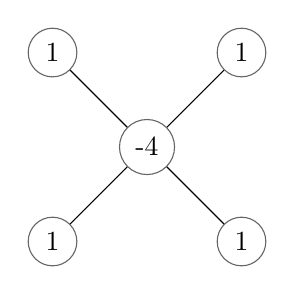
\begin{tikzpicture}

	\def \xone{0};
	\def \yone{0};
	\def \h{1.2}	

	\coordinate (M) at (\xone ,\yone);
	\coordinate (LU) at (\xone-\h ,\yone-\h);
	\coordinate (RU) at (\xone+\h ,\yone-\h);
	\coordinate (LO) at (\xone-\h ,\yone+\h);
	\coordinate (RO) at (\xone+\h ,\yone+\h);
	\draw (LU) -- (RO);
	\draw (RU) -- (LO);

	%draw nodes
	\node[circle,draw=black!60, fill=white!40] at (M) {-4};
	\node[circle,draw=black!60, fill=white!40] at (LO) {1};
	\node[circle,draw=black!60, fill=white!40] at (RO) {1};
	\node[circle,draw=black!60, fill=white!40] at (LU) {1};
	\node[circle,draw=black!60, fill=white!40] at (RU) {1};

		
	\end{tikzpicture}
\caption{rotated 5-point stencil}
\label{five_point_rot}
	
\end{figure}

			\item 9-point-stencil,  $2^{\text{nd}}$ order accurate and even $6^{\text{th}}$ order accurate for harmonic functions
				\begin{figure}[H]
	\center

	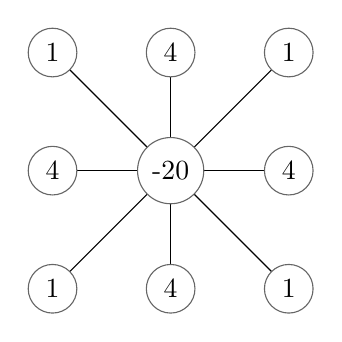
\begin{tikzpicture}
	
	\def \xone{0};
	\def \yone{0};
	\def \h{1.5}	

	\coordinate (M) at (\xone ,\yone);
	\coordinate (L) at (\xone-\h ,\yone);
	\coordinate (R) at (\xone+\h ,\yone);
	\coordinate (O) at (\xone ,\yone+\h);
	\coordinate (LU) at (\xone-\h ,\yone-\h);
	\coordinate (RU) at (\xone+\h ,\yone-\h);
	\coordinate (LO) at (\xone-\h ,\yone+\h);
	\coordinate (RO) at (\xone+\h ,\yone+\h);
	\coordinate (U) at (\xone ,\yone-\h);

	\draw (L) -- (R);
	\draw (U) -- (O);
	\draw (LU) -- (RO);
	\draw (RU) -- (LO);

	%draw nodes
	\node[circle,draw=black!60, fill=white!40] at (M) {-20};
	\node[circle,draw=black!60, fill=white!40] at (L) {4};
	\node[circle,draw=black!60, fill=white!40] at (R) {4};
	\node[circle,draw=black!60, fill=white!40] at (O) {4};
	\node[circle,draw=black!60, fill=white!40] at (U) {4};

	%draw diagonal nodes
	\node[circle,draw=black!60, fill=white!40] at (LO) {1};
	\node[circle,draw=black!60, fill=white!40] at (RO) {1};
	\node[circle,draw=black!60, fill=white!40] at (LU) {1};
	\node[circle,draw=black!60, fill=white!40] at (RU) {1};

	
	\end{tikzpicture}
	\caption{9-point stencil}
\label{nine_point}
	
\end{figure}

		\end{itemize}
\end{itemize}

\section{Finite difference on a grid}%
\label{sec:Finite difference on a grid}
Let $\Omega =(0, X_{E}) \times (0,Y_{E})$ and subdivide each interval into $N_{x}+1 / N_{y} + 1$ subintervals.

\[
\left.
	\begin{array}{c}
	N_{x} = 1 \\
	N_{y} = 2
\end{array}
\right\} \qquad
h_{x} = \frac{x_{E}}{N_{x}+1}, \quad h_{y}= \frac{y_{E}}{N_{y}+1}
.\] 

\begin{figure}[H]
	\center
\begin{tikzpicture}[scale=3]
		
		\def \xone{0};
		\def \yone{0};		
		% draw coordinate system
		\coordinate (A) at (\xone,\yone);
		
		\draw[\to] (A) -- ++(0,1);
		\draw[\to] (A) -- ++(1,0);
		\draw (A) ++(0.5,0) -- ++ (0,1);
		\draw (A) ++(1,0) -- ++ (0,1) -- ++(-1,0);
		\draw (A) ++(0,0.333) -- ++ (1,0);
		\draw (A) ++(0,0.666) -- ++ (1,0);
		\draw[red!60] (A) -- (A) ++ (0,0.333);
		\draw[blue!60] (A) -- (A) ++ (0.5,0);

        \fill[black,font=\footnotesize] (A)  ++(1,0) node[under] {$x_{E}$}
										(A)  ++(0,1) node[left] {$y_{E}$}
										(A)  ++(0.25,0) node[under] {$h_{x}$}
										(A)  ++(0,0.1666) node[left] {$h_{y}$};
                                        
\end{tikzpicture}

\caption{Visualization of Grid}
\label{example_grid}
\end{figure}

Each node (vertex) in this grid is assigned an index tuple
\[
	(x,y) = (ih_{x}, jh_{y}) \stackeq{\wedge} (i,j)
.\] 
for $i \in \{0,1, \ldots , N_{x}+1\}, j \in  \{0,1, \ldots , N_{y}+1\}$

We denote the value at the node $(i,j)$ by
\[
	u(x,y)=u(ih_{x},jh_{y})=:u_{i,j}
.\] 
This results in the discrete Laplace operator $(h=h_{x}=h_{y})$
\[
	\laplace_{h}^{(5)}u_{i,j}=\frac{1}{2}(u_{i+1,j}+u_{i-1,j} +u_{i,j+1}+ u_{i,j-1} - 4u_{i,j})
.\]

\section{Node ordering}%
\label{sec:Node ordering}
To form a linear system, the nodes $(i,j)$ have to be numbered consecutively, i.e. we have to use a map
\[
	l\colon \N^{d} \rightarrow \N
.\] 

Examples:

\begin{enumerate}[label=\alph{enumi})]
	\item  Lexicographical ordering
		\[
			l(i,j) = j \cdot (N_{x} + 2) + i 
			\quad\text{ or }\quad
			l(i,j) = i \cdot (N_{y} + 2) + j
		.\] 

		% TODO Plot 1
	\item Red-Black ordering (checkerboard ordering)

		\begin{enumerate}[label=\arabic{enumii})]
			\item neighbouring nodes get different color
			\item number each node lexicographically
		\end{enumerate}

		% TODO Plot 2 

		Question 1: How many colors do you need in 3D?

		Question 2: Does an analytic expression for $l(i,j)$ exist?
	\item Cache-aware ordering (Cluster nodes into connected groups)

		% TODO Plot 3
		
		This ordering scheme utilizes the fact, that data which is "located in a neighbourhood in memory respectively" can be accessed much quicker and thus fastens the operations used on the matrices.

	\item Wave front orderings (diagonal ordering)

		% TODO Plot 4
\end{enumerate}

\section{Assembling}%
\label{sec:Assembling}

For the Poisson equation
\[
-\laplace u = f
.\] 
we can assemble a linear system $Au=f$ by applying the discrete operator $\laplace_{h}^{(5)}$ instead of $\laplace$ and by evaluating in the grid nodes
\[
	\begin{array}{ccl}
	A = (a_{rs}) 
	\quad&\text{ with }\quad 
	&a_{r(i,j),s(i',j')}= \frac{1}{h^{2}}\begin{cases}
		4 &\text{,if } r=s \\
		-1 &\text{,if } \abs{i-i'} = 1 \text{ and } \abs{j-j'} = 0 \\
		-1 &\text{,if } \abs{i-i'} = 0 \text{ and } \abs{j-j'} = 1 \\
		0 &\text{,otherwise}
	\end{cases} \\ \\
	f = (f_{r}) 
	\quad&\text{ with }\quad
	&f_{r(i,j)}=f(ih, jh)=f(x_{i}, y_{i})
	\end{array}
\] 
\[
	 A \stackeq{\wedge} -\laplace_{h}^{(5)}
.\] 

\section{Boundary conditions}%
\label{sec:Boundary condition}
For Dirichlet boundary condition the value $u$ at boundary nodes is fixed.

A node is boundary node if
\[
i \in  \{0, N_{x}+1\} \quad\text{ or }\quad j \in  \{0,N_{y}+1\}
.\] 

And so $u_{i,j} = g_{i,j}$ if $(i,j)$ is a boundary node.

The boundary condition can be realized by eliminating rows/columns in the matrix, i.e. let $r=l(i,j)$ a boundary index

\begin{align*}
	f &\leftarrow f-A_{\ast,r}\cdot g_{i,j} \\
	A_{r,\ast} &\leftarrow \delta_{r,s} \\
	A_{*,r} &\leftarrow \delta_{r,s} \\
	f_{r} &\leftarrow g_{i,j}
\end{align*}

\[
A\cdot \underline{u} = \underline{f}  
.\] 
%TODO die Matrix sah anders aus.
%re-TODO bin nur nicht fertig geworden -.-
%\[
%A = \begin{pmatrix}
%	X& &X&0&X& &X \\
%	 &X& &\vdots& &X&  \\
%	X& &X&0&X& &X
%	\end{pmatrix}
%.\] 

\section{Structure of the matrix}%
\label{sec:Structure of the matrix}
(before eliminating the boundary conditions)
\begin{enumerate}[label=\alph{enumi})]
	\item Lexicographical ordering
		\[
		A= \frac{1}{h^{2}}
		\underbrace{
		\begin{bmatrix}
			[A_{0}] & [-I] &&& \\
			[-I] & [A_0] &&&\\
				 &&\ddots && \\
				 &&& [A_0] & [-I] \\
				 &&& [-I]& [A_0]
		\end{bmatrix}
		}_{N_{x}+2 \text{ blocks}}
		.\] 

		\[
		A_0 = \begin{bmatrix}
			4 & -1 &&& \\
			-1 & 4 & -1 && \\
			 & -1 & \ddots && \\
			 &&&\ddots & -1 \\
			 &&&-1 & 4
		\end{bmatrix}
		.\] 
	\item Red-Black ordering

		\[
			\begin{bmatrix}
				D_{r} & B \\
				B^{T} & D_{b}
			\end{bmatrix}
			\quad \text{with}\quad D_{r/b}=-\frac{1}{h^{2}}I_{r/b}
		.\] 
		B contains the values from the coupling of the nodes
\end{enumerate}

Variation of the PDE:
\[
\partial_{t}u- \laplace u=f
.\] 
Simple backward Euler scheme for $\partial_{t}$
\[
\frac{1}{\tau}u^{m+1}- \laplace u^{m+1} = f -\frac{1}{\tau}u^{m}
.\] 
with $u^{m} \equiv u(t^{m})$ with $0=t^{0}<t^{1}< \ldots  < t^{md}$ and $\tau:=t^{m+1}-t^{m}$.

The corresponding FD discretization reads:

\[
	\left(\frac{1}{\tau}I + A\right) u^{m+1} = f + \frac{1}{\tau}u^{m}
.\] 

\section{Properties of the linear system}%
\label{sec:Properties of the linear system}

\begin{definition}
\label{thm:typeOfMatrices}
	A matrix $A \in  \R^{n \times n}$ is called
	\begin{itemize}
		\item \underline{Z-matrix}, if $a_{ij}\leq 0\quad \forall i\neq j$
		\item \underline{symmetric positive definite}, if $A=A^{T}$ and $A>0$, i.e. $u^{T}Au>0\quad\forall u \in \R^{n} \setminus 0$
		\item \underline{positive definite} , if $A+A^{T}>0$
		\item \underline{M-matrix}, if $A$ is Z-matrix and $\Re(\lambda) > 0 \quad\forall \lambda \in \sigma (A)$
		\item \underline{M$_{0}$-Matrix}, if it is pos. def. and Z-matrix (M$_{0}$-matrix is an M-matrix)
	\end{itemize}
\end{definition}

\begin{definition}
\label{thm:adjacenyGraph}
Let $A$ be a (sparse) matrix. The graph $G_{A}=(V,E)$ with $E \subset V \times V$ is called \underline{adjacency graph} of $A$ if 
\begin{itemize}[label=]
	\item $V$ represents the $n$ unknowns/rows/columns
	\item $V=\{1, \ldots, n\}$
	\item $E=\{(i,j) \in  V \times V : a_{ij}\neq 0\}$
\end{itemize}
(The edges represent the relation: equations $i$ involves unknown $j$)
\end{definition}

\begin{definition}
\label{thm:irreducible}
A matrix $A$ is called \underline{irreducible} if for $G_{A}=(V,E)$:
\[
	\forall i,j \in V ~:~ \exists \text{ sequence of edges } (e_0, e_1, \ldots , e_{n}) \subset E
\] 
such that
\[
	e_0=(i, k_0), e_1=(k_0,k_1),\ldots , e_{m}=(k_{m-1},j) \quad \text{with } k_{j} \in V
.\] 

(All vertices are connected by a sequence of edges)
\[
	\mathcal{IR}:= \{A \in  \R^{n \times  n} | A \text{ is irreducible}\}
.\] 
\end{definition}

\begin{definition}
\label{thm:WDDmatrices}
\begin{align*}
	WDD:= &\left\{ A \in \R^{n \times n}, \abs{a_{j,j}}  \geq \sum_{i\neq j}^{}{\abs{a_{i,j}} } \quad \forall j \right\}  \\
		 = &\left\{ A \in R^{n \times }, \abs{a_{i,i}} \geq \sum_{i\neq j}^{}{\abs{a_{i,j}} } \quad \forall i \right\} 
\end{align*}
are the weakly diagonal dominant matrices.
\[
DD:= \left\{ A \in WDD, \exists j : ">" \right\} 
\] 
are diagonal dominant matrices.
\[
SDD := \left\{ A \in WDD, \forall j : ">" \right\} 
\] 
are the strictly diagonal dominant matrices.
\[
IDD := \left\{ A \in DD, A \text{ is irreducible} \right\} 
\] 
are the irreducible diagonal dominant matrices.
\end{definition}

\begin{theorem}(Gershgorin)
\label{thm:gershgorin}
Any eigenvalue $\lambda \in \sigma (A)$ is located in one of the closed discs in the complex plane centered at $a_{i,i}$ and having the radius
\[
	\rho_{i} = \sum_{\substack{j=0 \\ j \neq i}}^{n}{\abs{a_{i,j}} }
.\] 
In other words : 
\[
	\forall \lambda \in \sigma (A) \exists i \text{ such that } \abs{\lambda - a_{i,i}}  \leq \sum_{\substack{j=0 \\ j \neq i}}^{n}{\abs{a_{i,j}} }
.\] 
\end{theorem}

\begin{proof}
\label{thm:gershgorinproof}
	Let $x$ be an eigenvector associated to eigenvalue $\lambda$ and let $m$ be the index of the component with largest modulus in $x$.

	Scale $x$, s.t.
	\[
	\abs{x_{m}}  = 1 \text{ and } \abs{x_{i}} \leq 1 \quad \forall i \neq m
	.\] 
	Since $x$ is an eigenvector to $A$, we have
	\[
		(\lambda - a_{n,m}) x_{m} = - \sum_{\substack{j=1 \\ j \neq m}}^{n}{\abs{a_{m,j}} x_{j}}
	.\] 
	Taking the absolute value of this, we get
	\[
		\abs{\lambda - a_{m,m}}  \leq \sum_{j\neq m}^{}{\abs{a_{m,j}} \abs{x_{j}} } \leq \sum_{j\neq m}^{}{\abs{a_{m,j}} } = \rho_{m}
	.\] 
\end{proof}
\begin{figure}[H]
	\center
\begin{tikzpicture}[scale=3]
		
		\def \xone{0};
		\def \yone{0};		
		% draw coordinate system
		\coordinate (A) at (\xone,\yone);
		
		\draw[->] (A) ++ (0,-0.75) -- ++(0,1.5);
		\draw[->] (A) ++ (-0.5,0)-- ++(2.2,0);

		% a circle is easier to draw than another object
        \draw (A) ++(0.5,0) circle (0.4cm);
		\draw (A) ++(0.5,-0.05) -- ++(0,0.1);
        \draw (A) ++(1,0) circle (0.6cm);
		\draw (A) ++(1,-0.05) -- ++(0,0.1);

        \fill[black,font=\footnotesize] (A) ++(1.7,0) node[below] {Re}
										(A) ++(0,0.75) node[left] {Im};
                                        
\end{tikzpicture}

\caption{Example for Gershgorin discs}
\label{gerschgorin_discs}
\end{figure}

\begin{theorem}
\label{thm:gershgorinboundary}
	Let $A$ be irreducible and assume that an eigenvalue $\lambda$ lies on the boundary of the union of all Gershgorin discs. Then $\lambda$ lies on the boundary of all Gershgorin discs.
\end{theorem}

\begin{proof}
\label{thm:gershgorinboundaryproof}
	Iterate proof of \href{thm:gershgorinproof}{the last proof} along the connecting edges of any pairs of nodes. Do this for all pairs and you get the result.

	For more details, read the proof in some book.
	%TODO vlt Verweis hinzufügen.
\end{proof}

\begin{korollar}
\label{thm:gershgorinboundarycorollary1}
	If $A$ is strictly diagonal dominant or $A$ is irreducible diagonal dominant, then $A$ is non-singular.
\end{korollar}

\begin{proof}
\label{thm:gershgorinboundarycorollary1proof}
	\begin{enumerate}[label=\alph{enumi})]
		\item Assume $A \in SDD$.

			Then the Gershgorin discs exclude the origin. This means $\lambda =0$ cannot be an eigenvalue of $A$.

		\item Assume $A \in IDD$.

			Then if it is singular, the zero eigenvalue lies on the boundary of the union of the Gershgorin discs. Together with \href{thm:gershgorinboundary}{Theorem 2} this implies that the eigenvalue should be located on the boundary of all discs.
			\[
				\implies \abs{a_{j,j}} = \sum_{i \neq j}^{}{\abs{a_{i,j}} } \qquad \forall j=0, \ldots , n
			.\] 
			$\lightning$, since $A$ is diagonal dominant.
	\end{enumerate}
\end{proof}

\begin{korollar}
\label{thm:gershgorinboundarycorollary2}
	Let $A \in R^{n \times  n}$. If 
	\[
		A \in WDD \text{ and } A = A^{T} \text{ and } \text{diag}(A) \geq 0
	,\] 
	then $A$ is pos. semidefinit. 
\end{korollar}

\begin{proof}
\label{thm:gershgorinboundarycorollary2proof}
\begin{align*}
& A \text{ symmetric} \\
	\implies & \text{ eigenvalues are real} \\
	\overset{(\ast)}{\implies} & \forall \lambda  \in \sigma (A) : \lambda  \geq 0
\end{align*}
[with $(\ast) = \text{diag(A)} \geq 0 + A \in WDD + $ \href{thm:gershgorin}{Theorem 1}] 
\end{proof}

%\begin{summary}
\label{thm:summarymatrices}
$A = \laplace_{h}^{(5)}$ is 
\begin{itemize}
	\item symmetric $A = A^{T}$
	\item $A \in WDD$
	\item For Dirichlet boundary conditions we even have $A \in DD$
	\item $A$ is irreducible
	\item $\text{diag}(A) \geq 0$
	\item $\implies A$ is positive definit and $A$ is $M_0$-matrix and thus $M$-matrix.
\end{itemize}
%\end{summary}
